% IEEE's authorship policy does not allow AI tools to be listed as authors. For an IEEE
% submission, move Claude from the author block to the Acknowledgment, which already
% describes Claude's part in the work.
\documentclass[conference]{IEEEtran}
\usepackage{cite}
\usepackage{graphicx}
\usepackage{booktabs}
\usepackage{amsmath}
\usepackage{array}
\usepackage{url}

\begin{document}

\title{ImageNet-22k Pretraining, Augmentation, and Regularization: Where a ConvNeXt Recipe Departs from the MedMNIST+ Setup on TissueMNIST}

\author{
\IEEEauthorblockN{Isaiah R. Harville}
\IEEEauthorblockA{Independent Researcher}
\and
\IEEEauthorblockN{Claude}
\IEEEauthorblockA{Anthropic}
}

\maketitle

\begin{abstract}
MedMNIST+ trained ten pretrained networks on TissueMNIST, a set of 236,386 kidney-cortex
cell images in eight classes, with one shared setup: ImageNet-1k or self-supervised weights,
no data augmentation, plain cross-entropy, and early stopping on validation loss. Its best
TissueMNIST AUROC is 0.9535, a three-seed mean for DenseNet-121 trained end to end on
128-pixel images zero-padded to 224. We fine-tuned ConvNeXt-Small on the 224-pixel images
and the official split with a recipe that differs in six ways: supervised ImageNet-22k
pretraining, random resized crops and flips, label smoothing with stochastic depth and
stronger weight decay, a fixed 8-epoch cosine schedule with selection on validation
AUROC, an exponential moving average of the weights used only to select the epoch, and
flip averaging at test time. One run reached a test AUROC of 0.9630, with a 95\%
bootstrap interval of [0.9618, 0.9641] that lies above every published TissueMNIST value
we could source. Accuracy was 0.7772 against 0.7425 for the same baseline, so about one
test cell in five is still misclassified. Our input images are those of the MedMNIST+ 224-pixel runs, whose best AUROC is 0.9525,
so input size does not explain the gap. We ran no ablations, so we state each other
difference as a hypothesis with the run that would test it. The result is one seed, and
the bootstrap resamples images because TissueMNIST has no specimen identifiers.
\end{abstract}

\begin{IEEEkeywords}
TissueMNIST, MedMNIST+, kidney histology, cell classification, ConvNeXt, transfer
learning, data augmentation, bootstrap confidence intervals
\end{IEEEkeywords}

\section{Introduction}

MedMNIST+~\cite{doerrich2025medmnistplus} extended the MedMNIST v2
benchmark~\cite{yang2023medmnistv2} to images of 64, 128, and 224 pixels. It trained ten
networks on each 2D dataset at each size, in three training schemes and with three
seeds, under one fixed training setup. That design is good for comparing architectures.
It also means the benchmark says little about how much a different training recipe can
add to a given network.

TissueMNIST is the largest 2D MedMNIST dataset and among the hardest by accuracy. No
published method we found exceeds 0.75 accuracy on its eight classes, and the MedMNIST+
end-to-end AUROCs span 0.8644 to 0.9535~\cite{doerrich2025medmnistplus}. It is also
unusual in how its larger images are made: every TissueMNIST size is resized from the same
$32\times32$ projection, so the 224-pixel images hold no more detail than that
projection.

We report one model, ConvNeXt-Small~\cite{liu2022convnext} pretrained on ImageNet-22k,
fine-tuned end to end on the 224-pixel images with the recipe that our pipeline applies to
every MedMNIST 2D dataset. Its test AUROC interval lies above the published values. The
paper's purpose is to set out exactly what our recipe does differently from MedMNIST+,
since those differences are the candidate explanations. We take the MedMNIST+ setup from
its Method section and, where the paper is silent, from its public training code. We did
not ablate any difference, so we present each attribution as a hypothesis together with
the run that would test it.

\section{Related Work}

MedMNIST v2~\cite{yang2023medmnistv2} reported
ResNet-18 and ResNet-50 and three AutoML systems on 28-pixel images, with the ResNets
also run on the 28-pixel images upsampled to 224. Each value is a mean over at least three
trials. MedMNIST+~\cite{doerrich2025medmnistplus} evaluated VGG16, AlexNet, ResNet-18,
DenseNet-121~\cite{huang2017densenet}, and EfficientNet-B4 with ImageNet-1k weights, and
ViT-B/16 with ImageNet-1k, CLIP, DINO, EVA-02, and SAM weights. Each was trained end to
end, as a linear probe on frozen features, and as an 11-nearest-neighbor classifier on
frozen features. MedViT~\cite{manzari2023medvit} and MedViTV2~\cite{manzari2026medvitv2}
are hybrid convolution and transformer networks that report TissueMNIST results on images
resized to 224 pixels, without seeds or intervals. BBBC051, the source of TissueMNIST, is in the Broad Bioimage Benchmark
Collection~\cite{ljosa2012bbbc}. Woloshuk et al.~\cite{woloshuk2021kidney} classified its
cells from 3D stacks, so their numbers are not comparable.

\section{Data}
\label{sec:data}

\subsection{From BBBC051 to TissueMNIST}

The \texttt{medmnist} package describes TissueMNIST as 236,386 cells ``segmented from 3
reference tissue specimens'' in BBBC051~\cite{yang2023medmnistv2}. Each source image is a
$32\times32\times7$ gray-scale stack. MedMNIST takes the maximum over the seven slices and
resizes the $32\times32$ projection to $28\times28$. The official split, made ``with a
ratio of 7:1:2'', has 165,466 training, 23,640 validation, and 47,280 test images. The
eight classes are collecting duct and connecting tubule (CD/CNT), distal convoluted tubule
(DCT), glomerular endothelial cells (GEC), interstitial endothelial cells (IEC),
leukocytes, podocytes, proximal tubule segments (PT), and thick ascending limb (TAL). The
test split is imbalanced: CD/CNT has 15,165 images and GEC has 1,677.

The archives carry no patient or specimen identifiers. Our pipeline therefore treats each
image as its own patient and could not check the split for leakage. With all cells drawn
from three specimens and the split made at the cell level, test cells almost certainly
share a specimen with training cells. The benchmark measures generalization to new cells
from the same tissue, not to new donors.

\subsection{How the 224-pixel inputs are made}
\label{sec:pixels}

The MedMNIST+ notes in the MedMNIST
repository\footnote{\url{https://github.com/MedMNIST/MedMNIST/blob/main/on_medmnist_plus.md}} state that, after the maximum projection, ``for size
224x224, 128x128, and 64x64, we resize the source images into the target size''. The
notes do not name the interpolation method. The eight test images that our run publishes
vary smoothly between source pixels: from 31\% to 55\% of horizontally adjacent pixel
pairs are equal, where a nearest-neighbor enlargement by a factor of 7 would make at
least 6 in 7 (86\%) equal. The resize therefore interpolates. A 224-pixel TissueMNIST
image is a $32\times32$ projection enlarged seven times. It is not a higher-resolution
view of the cell.

The MedMNIST+ training code loads the subset at the chosen size with
\texttt{as\_rgb=True}, which repeats the gray channel three times, normalizes it with the
network's default mean and standard deviation, and then pads it with zeros to
$224\times224$. For the best baseline, DenseNet-121 at 128 pixels, this places the
$128\times128$ image in the center with a 48-pixel border on each side. Because the
padding comes after normalization, the border equals the ImageNet channel means in pixel
terms rather than black. At 224 pixels nothing is padded. The authors chose padding over
interpolation citing Hashemi~\cite{hashemi2019padding}, whose comparison they summarize as showing no
effect on accuracy and shorter training.

Our data module downloads the official \texttt{tissuemnist\_224.npz} archive, checks its
MD5 (\texttt{b077128c\ldots}) against the \texttt{medmnist} package metadata, and serves
the arrays as stored. At evaluation the only resize is a \texttt{Resize(224)}, which
torchvision returns unchanged for a 224-pixel image. Our inputs are therefore the same
images as those of the MedMNIST+ 224-pixel runs, and differ from the 128-pixel baseline
only in the enlargement factor and in its border.

\section{Method}
\label{sec:method}

\begin{table*}[t]
\caption{Training setup of MedMNIST+~\cite{doerrich2025medmnistplus} for its end-to-end
TissueMNIST runs and of our run. P: stated in the MedMNIST+ Method section. C: read
from its public repository at commit \texttt{b67b772} where the paper is silent
(\texttt{train.py}, \texttt{evaluate.py}, \texttt{config.yaml}, \texttt{utils.py}).
N: MedMNIST+ notes in the MedMNIST repository. S: Supplementary Table~S12. Our values come from
the run's resolved \texttt{config.yaml} and \texttt{scripts/medmnist\_recipes.py}. Rows marked
$\ast$ differ.}
\label{tab:setup}
\centering
\footnotesize
\renewcommand{\arraystretch}{1.08}
\begin{tabular}{@{}l>{\raggedright\arraybackslash}p{0.40\textwidth}>{\raggedright\arraybackslash}p{0.36\textwidth}@{}}
\toprule
Item & MedMNIST+ & Ours \\
\midrule
Network$^\ast$ & DenseNet-121 for the best result, among ten networks (P, S) & ConvNeXt-Small, 49,457,768 parameters \\
Pretraining$^\ast$ & ImageNet-1k (P); timm default tag, which timm 1.0.31 resolves to \texttt{ra\_in1k} (C) & ImageNet-22k, then ImageNet-1k (\texttt{convnext\_small.fb\_in22k\_ft\_in1k}) \\
Scheme & end to end, also linear probe and $k$-NN (P) & end to end \\
Input image & 128 px resized from $32\times32$, zero-padded to 224 (P, N, C); or 224 px resized from $32\times32$ & 224 px resized from $32\times32$, as released (N) \\
Gray input$^\ast$ & repeated to 3 channels, network's default mean and std (C) & 1 channel, stem filters summed, mean 0.449, std 0.226 \\
Augmentation$^\ast$ & none stated (P); none in code (C) & random resized crop, area 0.7--1.0, aspect 3:4--4:3; horizontal and vertical flips \\
Optimizer$^\ast$ & AdamW, lr $10^{-4}$, batch 64 (P); default weight decay, 0.01 in timm 1.0.31 (C) & AdamW, lr $10^{-4}$, batch 64, weight decay 0.05 \\
Schedule$^\ast$ & cosine, one cycle (P) over 100 epochs to 0, per epoch (C) & cosine over 8 epochs to $10^{-6}$, per epoch \\
Epochs and stopping$^\ast$ & up to 100, early stopping on validation (P); stop after 5 epochs without lower validation loss (C) & fixed 8 epochs, 20,688 steps \\
Selection$^\ast$ & lowest validation loss (C) & highest validation AUROC \\
Loss$^\ast$ & cross-entropy (P) & cross-entropy, label smoothing 0.1 \\
Regularization$^\ast$ & none stated & stochastic depth 0.2 \\
Weight averaging$^\ast$ & none & EMA, decay 0.99952; used for validation, not saved \\
Test-time augmentation$^\ast$ & none in code (C) & mean softmax of image and horizontal mirror \\
Precision$^\ast$ & fp32, no autocast in code (C) & bf16 mixed \\
Seeds$^\ast$ & 3, mean reported (P) & 1 \\
AUROC, accuracy & macro one-vs-rest; argmax, through the \texttt{medmnist} evaluator (C) & macro one-vs-rest; argmax \\
Hardware & one NVIDIA RTX A5000 (P) & one NVIDIA GeForce RTX 4070 Ti \\
\bottomrule
\end{tabular}
\end{table*}

Table~\ref{tab:setup} sets the two setups side by side. The repository of MedMNIST+ does
not pin its library versions, so where a default depends on the version we give the value
in the version we checked. The two setups share the optimizer family, learning rate, batch
size, schedule shape, and, at 224 pixels, the input images. Most other items differ.

\subsection{Network}

The network is timm's~\cite{wightman2019timm}
\texttt{convnext\_small.fb\_in22k\_ft\_in1k}: ConvNeXt-Small~\cite{liu2022convnext}
pretrained on ImageNet-22k and then fine-tuned on ImageNet-1k~\cite{deng2009imagenet},
with a new eight-way head. timm adapts the pretrained stem to one input channel by summing
its RGB filters. Our gray mean and standard deviation, 0.449 and 0.226, are the averages of
the ImageNet channel values. Summed filters on one normalized channel are therefore close
to the MedMNIST+ approach of repeating the channel and normalizing each copy, and we do not
expect this difference to matter. We set the stochastic depth~\cite{huang2016stochastic}
rate to 0.2.

\subsection{Training}

We trained all layers for 8 epochs with batch size 64, which is 2,586 steps per epoch. The
optimizer is AdamW~\cite{loshchilov2019adamw} with learning rate $10^{-4}$ and weight
decay 0.05. A cosine schedule~\cite{loshchilov2017sgdr}, stepped once per epoch, lowered
the rate from $10^{-4}$ in the first epoch to $4.8\times10^{-6}$ in the eighth. The loss is
cross-entropy with label smoothing~\cite{szegedy2016inception} of 0.1. Training used bf16
mixed precision. Training augmentation is a random resized crop back to 224 pixels,
covering 70\% to 100\% of the image area with aspect ratios from 3:4 to 4:3, followed by
independent horizontal and vertical flips with probability 0.5 each. Cells have no
preferred orientation, so the recipe keeps flips for this dataset. At evaluation the model
averages the softmax probabilities of each image and its horizontal mirror.

We kept an exponential moving average (EMA) of the weights with decay 0.99952. The recipe generator sets the
decay to $1-10/S$ for $S=20{,}688$ total steps, a horizon of about 2,100 steps or 0.8
epochs. Lightning's \texttt{EMAWeightAveraging} callback swaps the averaged weights in for
each validation pass, so the per-epoch validation AUROC, and hence the epoch selection, used
the EMA weights. The callback writes the averaged weights into a checkpoint only from its
save hook. Lightning~2.6.6 skips callback save hooks when
\texttt{save\_weights\_only} is true, which is our pipeline's setting. The saved checkpoint,
and so every test number in this paper, holds the raw weights at the end of the selected
epoch. EMA influenced only which epoch was kept.

The recipe comes from \path{scripts/medmnist_recipes.py}, which writes one configuration
for all twelve MedMNIST 2D datasets. They differ only in epoch count and in whether flips
are used. No hyperparameter search on TissueMNIST is recorded.

\section{Evaluation Protocol}

AUROC is the macro average of the eight one-vs-rest AUROCs, the definition the
\texttt{medmnist} evaluator and the MedMNIST+ code use. Accuracy is the share of test
images whose most probable class is the true class. The MedMNIST+ paper describes its
accuracy as taken at ``a fixed operating point of 0.5'', but its code passes softmax
outputs to the \texttt{medmnist} evaluator, which takes the argmax for multiclass tasks. The
two accuracies are therefore comparable. We also report balanced accuracy and macro
average precision (AUPRC). AUROC and AUPRC come from scikit-learn~\cite{pedregosa2011sklearn}
in float64.

Each interval is a 95\% percentile bootstrap with 1,000 replicates and seed 0. The
pipeline resamples whole patients when identifiers exist, following the clustered
bootstrap~\cite{field2007bootstrap}. With none, \texttt{evaluation.py} sets the unit to
single images, and \texttt{metrics.json} records ``sample (no patient IDs)''. Cells of one
specimen share staining and tissue properties, so these intervals cover test sampling
among images and are likely narrower than an interval over specimens. They do not cover
variation between training runs.

The checkpoint was the epoch with the highest validation AUROC among eight end-of-epoch
evaluations. No threshold or calibration step applies to this multiclass task. The test
split was scored once, after selection.

The run trained at commit \texttt{ab39eb9}. Its \texttt{metrics.json} and predictions were
then regenerated from the saved checkpoint, with the same selection, at commit
\texttt{e9f733f}. Between the two, the pipeline switched its AUROC and AUPRC from
torchmetrics in float32 to scikit-learn in float64. All numbers below come from the
rescored files, except the per-epoch curves, which were logged during training.

\section{Results}
\label{sec:results}

\begin{table*}[t]
\caption{TissueMNIST test results on the official split. Our row gives 95\% percentile
bootstrap intervals over test images. Baseline values are copied from the cited tables,
which publish no intervals or predictions. ``Runs'' is the number of seeds or trials
averaged (n.s.: not stated). An arrow marks a resize. ``32'' is the $32\times32$ maximum
projection.}
\label{tab:main}
\centering
\footnotesize
\setlength{\tabcolsep}{4pt}
\begin{tabular}{@{}llllll@{}}
\toprule
Method & Network input & Runs & AUROC & Accuracy & Source \\
\midrule
ConvNeXt-S, end to end (ours) & 32 $\rightarrow$ 224 & 1 & \textbf{0.9630} [0.9618, 0.9641] & \textbf{0.7772} [0.7739, 0.7811] & this work \\
DenseNet-121, end to end & 32 $\rightarrow$ 128, padded to 224 & 3 & 0.9535 & 0.7425 & \cite{doerrich2025medmnistplus}, Table~S12 \\
DenseNet-121, end to end & 32 $\rightarrow$ 224 & 3 & 0.9525 & 0.7408 & \cite{doerrich2025medmnistplus}, Table~S12 \\
MedViT-S & resized to 224 & n.s. & 0.952 & 0.731 & \cite{manzari2023medvit}, Table~3 \\
MedViTV2-L & resized to 224 & n.s. & 0.943 & 0.716 & \cite{manzari2026medvitv2}, Table~5 \\
AutoKeras & 28 & $\geq 3$ & 0.941 & 0.703 & \cite{yang2023medmnistv2}, Table~3 \\
ResNet-18 & 28 $\rightarrow$ 224 & $\geq 3$ & 0.933 & 0.681 & \cite{yang2023medmnistv2}, Table~3 \\
ResNet-50 & 28 $\rightarrow$ 224 & $\geq 3$ & 0.932 & 0.680 & \cite{yang2023medmnistv2}, Table~3 \\
ResNet-50 & 28 & $\geq 3$ & 0.931 & 0.680 & \cite{yang2023medmnistv2}, Table~3 \\
ResNet-18 & 28 & $\geq 3$ & 0.930 & 0.676 & \cite{yang2023medmnistv2}, Table~3 \\
Google AutoML Vision & 28 & $\geq 3$ & 0.924 & 0.673 & \cite{yang2023medmnistv2}, Table~3 \\
auto-sklearn & 28 & $\geq 3$ & 0.828 & 0.532 & \cite{yang2023medmnistv2}, Table~3 \\
\bottomrule
\end{tabular}
\end{table*}

\subsection{Comparison with published results}

Table~\ref{tab:main} places our run against every baseline in the project's
\texttt{baselines.yaml}, each checked against its source table. Our test AUROC is 0.9630
[0.9618, 0.9641]. The highest published value, 0.9535 for MedMNIST+ DenseNet-121 at 128
pixels, is 0.0083 below our lower bound. The MedMNIST+ DenseNet-121 run on the same
224-pixel images as ours scored 0.9525. MedMNIST+ reports standard deviations of 0.0007
and 0.0004 across seeds for those two rows. Our accuracy is 0.7772 [0.7739, 0.7811]
against 0.7425 and 0.7408. Both baselines lie below our intervals for both metrics. No baseline publishes per-image predictions, so we could not run a paired test.

Accuracy stays low in absolute terms. About 22\% of test cells are misclassified, and
balanced accuracy, the mean of per-class recall, is 0.7093 [0.7041, 0.7150]. Macro AUPRC is
0.7882 [0.7826, 0.7941]. On validation the saved checkpoint scores AUROC 0.9620 [0.9600,
0.9639] and accuracy 0.7810 [0.7754, 0.7864], close to its test scores.

\subsection{Per-class results}

Fig.~\ref{fig:perclass} gives the one-vs-rest AUROC of each class. Seven classes lie
between 0.9598 (TAL) and 0.9776 (GEC). DCT is the exception at 0.9297 [0.9243, 0.9351],
with a recall of 0.412. At the argmax decision, 30\% of DCT cells are predicted as CD/CNT and 14\% as TAL, both tubule segments that adjoin
the distal convoluted tubule. The second large confusion is between the two glomerular
classes: 24\% of podocytes are predicted as glomerular endothelial cells, and 14\% of
glomerular endothelial cells as podocytes. GEC and podocytes have one-vs-rest AUROCs above
0.97 but recalls of 0.722 and 0.589. The model separates these cells well from the other
six classes and poorly from each other.

\begin{figure}[t]
\centering
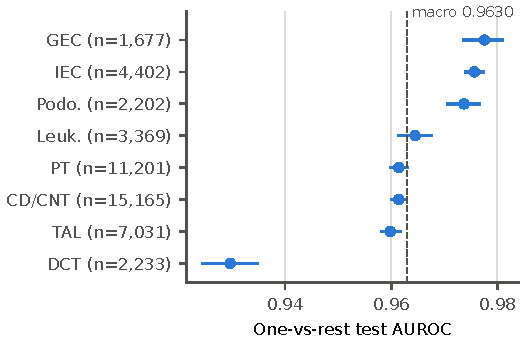
\includegraphics[width=\columnwidth]{figures/per_class_auroc.pdf}
\caption{One-vs-rest test AUROC per class, sorted, with 95\% bootstrap intervals over
test images. The dashed line is the macro mean.}
\label{fig:perclass}
\end{figure}


\subsection{Training dynamics}
\label{sec:dynamics}

Fig.~\ref{fig:curves} shows the per-epoch history. The logged validation AUROC, computed
on the EMA weights, rose from 0.9253 after the first epoch to 0.9641 after the seventh and
was 0.9638 after the eighth, so selection kept the seventh epoch. Training loss fell every
epoch, from 1.226 to 0.871. Rescoring the saved raw weights of the seventh epoch gives a
validation AUROC of 0.9620 and accuracy of 0.7810, against 0.9641 and 0.7869 logged for
the EMA weights. Most of that 0.0021 gap in AUROC is the difference between the averaged
and the raw weights, since the change of metric library moves AUROC by at most about
$10^{-4}$ according to the pipeline's notes. The EMA weights may therefore have scored
higher on test than the numbers we report, but they were not saved, and we cannot check.
Validation AUROC stayed within 0.0007 over the last three epochs, so the 8-epoch budget
ended near a plateau.

\begin{figure*}[t]
\centering
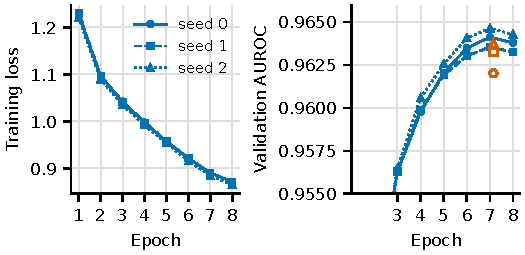
\includegraphics[width=\textwidth]{figures/training_curves.pdf}
\caption{Training loss and validation metrics per epoch, as logged during training. The
validation curves used the EMA weights. Open squares mark the saved raw weights of the
selected epoch, rescored on validation. The dashed line marks the selected epoch.}
\label{fig:curves}
\end{figure*}

\section{Discussion}

\subsection{Which differences plausibly matter}

Every item marked in Table~\ref{tab:setup} changed at once, so no single one can be
credited with the gain of 0.0095 in point AUROC over the 128-pixel baseline. Some can be
set aside with evidence already in hand. For the others we give our reading and the run
that would test it. Each run below should use three seeds, so that its mean can be set
against the MedMNIST+ means.

\emph{Input size and framing.} This is the least likely explanation. Our input images are
the same as those of the MedMNIST+ 224-pixel runs, and their DenseNet-121 on those images
scored 0.9525, below the 0.9535 it scored at 128 pixels with padding. MedMNIST+ does show
that scale matters on this dataset: its DenseNet-121 rose from 0.9247 at 28 pixels to
0.9535 at 128, although every size comes from the same $32\times32$
projection~\cite{doerrich2025medmnistplus}. The gain from enlarging the cell appears to stop
by 128 pixels. The gray-channel handling is nearly the same function at initialization
(Section~\ref{sec:method}). No run is needed to set these aside.

\emph{Test-time flip averaging.} This is the cheapest to measure. Rescoring the released
checkpoint without the mirrored view needs no training.

\emph{Pretraining and architecture.} Our backbone saw ImageNet-22k labels before
ImageNet-1k, and larger pretraining sets have improved transfer to small target
datasets~\cite{kolesnikov2020bit}. ConvNeXt-Small is also a newer and larger network than
DenseNet-121. Among the MedMNIST+ end-to-end networks at 224 pixels, AUROC spans only
0.9220 to 0.9525~\cite{doerrich2025medmnistplus}, so architecture alone has moved this
benchmark by a few thousandths at the top. Two runs would separate pretraining from
architecture: our recipe with \texttt{convnext\_small.fb\_in1k}, and our recipe with
DenseNet-121 and ImageNet-1k weights.

\emph{Augmentation.} MedMNIST+ trains without augmentation. With 165,466 training images
this dataset is large, so overfitting is less of a concern than on small MedMNIST
datasets, but each image is a blurred, low-detail cell, and crops and flips change both its
position and orientation. In our view augmentation and pretraining are the two most likely
contributors. The test is our recipe with the crop and flips removed.

\emph{Regularization.} Label smoothing, stochastic depth of 0.2, and weight decay of 0.05
all act against overfitting, and their effects overlap with those of augmentation. One run
per component, each removed in turn, would measure them.

\emph{Schedule and stopping.} MedMNIST+ sets its cosine schedule over 100 epochs and stops
after five epochs without a lower validation loss. If training stops in the first 20
epochs, the learning rate is still above 90\% of its initial value, so the network is never
trained at a low rate. Our schedule reaches $4.8\times10^{-6}$ in its last epoch. Selection
also differs: lowest validation loss against highest validation AUROC, which can pick
different epochs. The test is our network under the MedMNIST+ schedule and stopping rule.

\emph{Weight averaging and precision.} EMA changed which epoch we kept and nothing else,
since the saved weights are raw. Validation AUROC stayed within 0.0007 over the last three
epochs, so the selection had little room to matter. We have no reason to expect bf16
to raise accuracy over fp32.

The most informative single experiment would reproduce the MedMNIST+ DenseNet-121 setup
in our pipeline, so that a paired test on the same test images measures the whole gap.

\subsection{Limitations}

We trained one seed, while the baselines are means of three. Our bootstrap interval
covers test sampling, not run-to-run variation. The MedMNIST+ seed standard deviations for
DenseNet-121 are small next to our margin of 0.0083, but we cannot assume ConvNeXt varies
as little until we train more seeds. The interval resamples images. Cells from one specimen
are correlated, so it is likely too narrow, and with three specimens a specimen-level
interval would not be informative either. The split is made at the cell level across three
specimens, so the result says nothing about new donors, staining, or microscopes. All selection used validation data only, and the test split was scored once. How the
8-epoch budget was chosen is not recorded.
The reported numbers come from the raw weights, and the EMA weights that guided selection
were not saved. 
Accuracy below 0.78 and a DCT recall of 0.412 mean the model would mislabel many cells.
This is a research model trained on a benchmark. It is not a medical device and has not
been evaluated for any clinical or laboratory use.

\section{Reproducibility and Licensing}
\label{sec:repro}

The run trained from a clean tree at commit
\texttt{ab39eb9758be4bb65d091fad1d98b521edfbf837} with the command
\path{uv run opendiagnostics fit -c models/tissuemnist-convnext/config.yaml}
on one NVIDIA GeForce RTX 4070 Ti under Windows 11, with Python 3.12.16, PyTorch
2.15.0~\cite{paszke2019pytorch} (CUDA 13.2), Lightning 2.6.6~\cite{falcon2020lightning},
timm 1.0.31, and \texttt{medmnist} 3.0.2. The run record spans 98 minutes. Seeds were 0,
and Lightning ran with \texttt{deterministic: warn} because several CUDA backward passes
lack deterministic kernels, so a GPU rerun may differ slightly. Metrics and predictions were rescored from the saved checkpoint, also from a clean tree,
at commit \texttt{e9f733fd5507fabc0a1f6bbd223937069d23e7a2}. The resolved
configuration, run record, per-epoch history, split membership, metrics, and per-image
validation and test predictions are in
\path{models/tissuemnist-convnext/runs/20261126-200655-ab39eb97} of
\url{https://github.com/isaiah-harville/opendiagnostics}. The 198~MB checkpoint, SHA-256
\texttt{ebb44652\ldots b64adef}, is at
\url{https://diagnostics.harville.dev/opendiagnostics-weights/tissuemnist-convnext/20261126-200655-ab39eb97/checkpoint.ckpt}.
The figures are drawn from the committed run files by
\path{papers/tissuemnist/make_figures.py} with matplotlib~\cite{hunter2007matplotlib},
which also recomputes the test AUROC and accuracy from the predictions.

BBBC051 images and ground truth are licensed under Creative Commons Attribution 3.0
Unported. MedMNIST declares CC BY 4.0 for TissueMNIST. Both permit redistribution with
attribution, so we publish the weights, the predictions, and eight example test images.

\section{Conclusion}

A ConvNeXt-Small fine-tuned with ImageNet-22k pretraining, augmentation, regularization,
a short cosine schedule, and flip averaging reached a TissueMNIST test AUROC whose interval
lies above the published values. The comparison with MedMNIST+ rules out input size as the
cause, because the images are the same. It leaves pretraining, architecture, augmentation,
regularization, and the schedule as candidates. The next steps are two more seeds, the
rescoring without flip averaging, the ablations named above, and a reproduction of the
DenseNet-121 baseline in our pipeline for a paired test.

\section*{Acknowledgment}

Claude, an AI model developed by Anthropic, took part in this work. It helped design and
run the experiments, analyzed the results, generated the figures, and drafted and revised
the text. Isaiah R. Harville reviewed the work and is responsible for its content. We
thank the creators of BBBC051 and of MedMNIST for releasing their data under open
licenses.

\bibliographystyle{IEEEtran}
\bibliography{refs}

\end{document}
